\scanpage{34}
Lorsque cette condition est satisfaite, on définit un nouveau diagramme (dont le type se déduit de façon évidente du type de diagrammes $I$, des ensembles ordonnés par incidence \deleted{des} $\Phi_i$ des feuilles des espaces $X_i$, et des morphismes d'ensembles ordonnés \deleted{$\unsure{\Phi|\mathcal X}$} $\Phi_i\unsure{-|\to}\Phi_j$ définis par les \deleted{flèches} applications $X_i\to X_j$ définies par les flèches du diagramme $I$ -- d'où un diagramme \inserted{$(\Phi_i)_{i\in I}$} de type $I$ d'ensembles ordonnés $\ldots$), par les applications $\overline F_{i,\alpha}\unsure{-|\to}\overline F_{j,\beta}$ entre feuilles \uline{fermées} induites par les $X_i\unsure{-|\to}X_j$.

Ceci dit, le \deleted{système \unsure{diagramme}}\inserted{système} des partitions des $X_i$ est dit \uline{équisingulier} (relativement au diagramme donné $\mathcal X=(X_i)_{i\in I}$) si \inserted{\unsure{(il est admissible, et si)}} le diagramme \deleted{des}\inserted{précédent} \deleted{$\unsure{F}$} applications entre feuilles fermées est équisingulier le long de toute feuille (\unsure{entrante}) de tout $X_i$.

\margin{Un système de partitions est dit ``privilégié'' s'il est équisingulier et si de plus toutes les feuilles de tous les $X_i$ sont des \uline{variétés} (sans bord).}
\figure{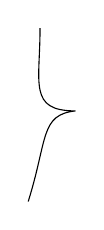
\begin{tikzpicture}[x=1cm,y=1cm]\draw (0,2.2) .. controls (0,1.5) and (-.15,1.15) .. (.45,1.15) .. controls (0,1.1) and (.1,.8) .. (-.15,0);\end{tikzpicture}}
\figure{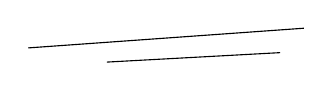
\begin{tikzpicture}[x=1cm,y=1cm]\draw (0,.18)--(3.5,.43);\draw (1,.0)--(3.2,.12);\end{tikzpicture}}

On suppose maintenant que le contexte soit linéaire (ou algébrique, ou analytique) par \uline{morceaux}.

\uline{Conjecture 1} Tout espace $X$ admet une partition \deleted{équisingulière}\inserted{privilégiée}. Parmi toutes les partitions \deleted{équisingulières}\inserted{privilégiées} de $X$, il en est une plus grossière que toutes les autres (appelée ``canonique'').
\mspage{35}
